\documentclass[tikz,border=5pt]{standalone}
\usepackage{tikz}
\usepackage{amsmath}
\usetikzlibrary{arrows.meta,positioning}
\definecolor{nebula}{HTML}{6366F1}
\definecolor{spark}{HTML}{14B8A6}
\definecolor{ink}{HTML}{334155}
\begin{document}
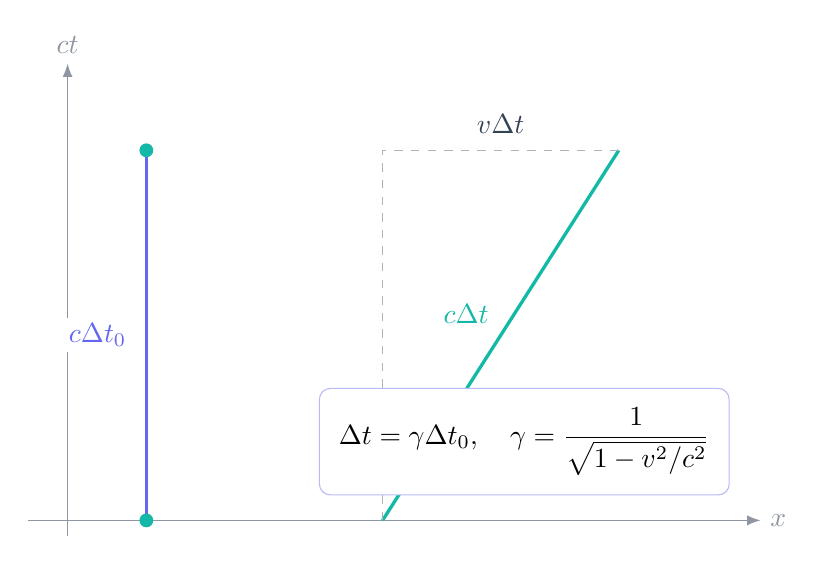
\begin{tikzpicture}[font=\sffamily,>=Latex,x=1cm,y=1cm]
  \draw[->,ink!55] (-.5,0)--(8.8,0) node[right] {$x$};
  \draw[->,ink!55] (0,-.2)--(0,5.8) node[above] {$ct$};
  \draw[very thick,nebula] (1,0)--(1,4.7);
  \fill[spark] (1,0) circle (2.5pt);
  \fill[spark] (1,4.7) circle (2.5pt);
  \node[fill=white,inner sep=2pt,text=nebula,left=5pt] at (1,2.35) {$c\Delta t_0$};
  \draw[very thick,spark] (4,0)--(7,4.7);
  \draw[dashed,ink!40] (4,0)--(4,4.7)--(7,4.7);
  \node[fill=white,inner sep=2pt,text=spark,above left=3pt] at (5.5,2.35) {$c\Delta t$};
  \node[fill=white,inner sep=2pt,text=ink,above=4pt] at (5.5,4.7) {$v\Delta t$};
  \node[draw=nebula!45,rounded corners=4pt,fill=white,inner sep=7pt] at (5.8,1.0)
    {$\displaystyle \Delta t=\gamma\Delta t_0,\quad \gamma=\frac1{\sqrt{1-v^2/c^2}}$};
\end{tikzpicture}
\end{document}
